\subsection{Оптические вычислители}\label{sec:OpticalCalcs}
Один из методов решения проблем описанных в \ref{sec:ANN} -- это делегирование задач отдельным вычислительным единицам. Как правило, подобные вычислительные единицы направлены на решение узкого спектра задач, например проекция трёхмерных данных на плоскость. Это позволяет эффективно изменить их архитектуру и способ работы с памятью. Ярким примером такого решения является графический процессор (ГП, GPU). Его основная задача -- это параллельная обработка большого массива данных. На рисунке \ref{ris:PerfomanceGPUCPU} изображена зависимость максимальной скорости вычислений в зависимости от года выпуска чипа, поэтому его можно использовать для сравнения производительности процессоров и графических процессоров в параллельной обработке информации. Видно, что разрыв производительности составляет от 2 до 8 раз, в зависимости от типа процессоров.
\par
Последнее время набирает популярность использование оптических устройств для ускорения или увеличение эффективности исполнения задач. Такие вычислители являются аналоговыми, чаще всего выполняют очень узкий спектр задач на скорости ограниченной лишь электронными частями схемы \cite{solli2015analog}, могут предоставлять высокий параллелизм обработки за счёт ортогональности излучения с различными длинами волн \cite{mcmahon2023physics}, а также, могут обеспечить низкое энергопотребление \cite{wu2022analog}. Существует множество исследований и оптических схем, выполняющих описанные ниже задачи.





\paragraph{Оптические корреляторы}
Оптический коррелятор -- это оптическое устройство производящее свёртку изображения с ядром. Существуют два основных метода оптической свёртки: $4f$ схема - VLC (Vander Lugt Correlator) коррелятор \cite{lugt1964signal}, изображённый на рисунке \ref{ris:VLC}, и JTC (Joint Trnsform Correlator) коррелятор \cite{weaver1966technique}, изображённый на рисунке \ref{ris:VLC}.
\begin{figure}[htbp]
	\centering{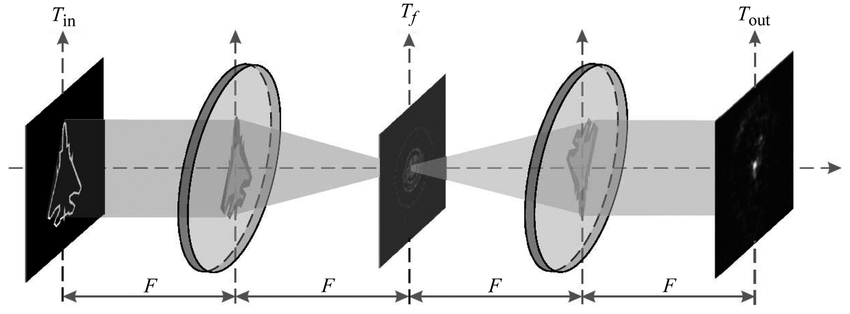
\includegraphics[width=0.8\linewidth]{figures/VLC.png}}
	\caption{Оптическая схема VLC коррелятора. Источник: \cite{goncharov2019features}.}
	\label{ris:VLC}
\end{figure}
\begin{figure}[htbp]
	\centering{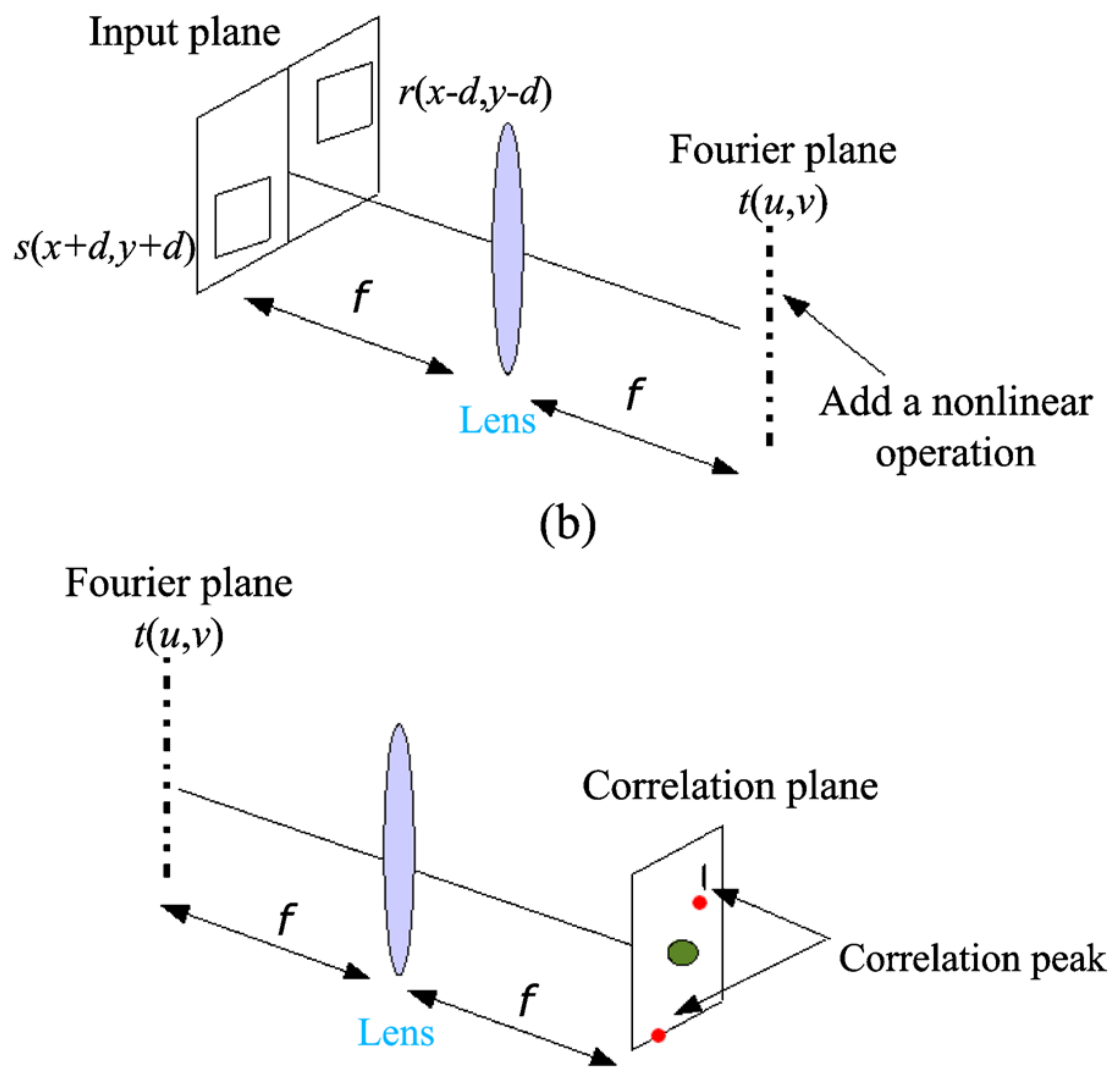
\includegraphics[width=0.65\linewidth]{figures/JTC.png}}
	\caption{Оптическая схема JTC коррелятора. Источник: \cite{alfalou2009optical}.}
	\label{ris:JTC}
\end{figure}
Принцип работы VLC коррелятора основан на теореме о свёртке: свёртка двух функций -- это обратное Фурье преобразование произведения их Фурье образов. В этой схеме (рисунок \ref{ris:VLC}), первая линза создаёт Фурье образ \cite{goodman2005introduction} на модуляторе, после прохождения этого модулятора, поле становится эквивалентно умножению Фурье образов изображения и ядра. В дальнейшем вторая линза осуществляет дополнительное преобразование Фурье, что эквивалентно, отражению вдоль каждой оси результата обратного Фурье преобразования.
Принцип работы JTC коррелятора (рисунок \ref{ris:JTC}) основан на том, что нелинейная функция от Фурье образа совмещённого изображения содержит член, пропорциональный произведению этих Фурье образов. Математические выражения, доказывающие это, приведены в последовательности уравнений \ref{eq:JTC1}, \ref{eq:JTC2}, \ref{eq:JTC3}, \ref{eq:JTC4}, \ref{eq:JTC5}, где символ $\bullet$ обозначает свёртку.
\begin{equation}\label{eq:JTC1}
	\left|\mathcal{F}\left(f(x,y) + g(x-b,y)\right)\right|^2 
	=
	\left|\mathcal{F}\left(f(x,y)\right) + \mathcal{F}\left(g(x,y)\right)e^{-ik_xb}\right|^2,
\end{equation}
\begin{equation}\label{eq:JTC2}
	\left|\mathcal{F}\left(f(x,y)\right) + \mathcal{F}\left(g(x,y)\right)e^{-ik_xb}\right|^2
	=
	\begin{matrix}
		+ \left|\mathcal{F}\left(f(x,y)\right)\right|^2 + \left|\mathcal{F}\left(g(x,y)\right)\right|^2 \\
		+ \mathcal{F}\left(f(x,y)\right)\mathcal{F}\left(g(x,y)\right)^*e^{+ik_xb} \\
		+ \mathcal{F}\left(f(x,y)\right)^*\mathcal{F}\left(g(x,y)\right)e^{-ik_xb}
	\end{matrix}.
\end{equation}
Учитывая, что:
\begin{equation}\label{eq:JTC3}
	\mathcal{F}^{-1}\left(
	\left|\mathcal{F}\left(f(x,y)\right)\right|^2
	\right)
	=
	\mathcal{F}^{-1}\left(
	\mathcal{F}\left(f(x,y)\right)\mathcal{F}\left(f^*(x,y)\right)
	\right)
	=
	f(x,y) \bullet f^*(x,y),
\end{equation}
\begin{equation}\label{eq:JTC4}
	\mathcal{F}^{-1}\left(
	\mathcal{F}\left(f(x,y)\right)\mathcal{F}\left(g(x,y)\right)^*e^{+ik_xb}
	\right)
	=
	(f(x,y) \bullet g^*(x,y))(x+b,y).
\end{equation}
Получим итоговое выражение:
\begin{equation}\label{eq:JTC5}
	\left|\mathcal{F}\left(f(x,y) + g(x-b,y)\right)\right|^2 
	=
	\begin{matrix}
		+ f(x,y) \bullet f^*(x,y) + g(x,y) \bullet g^*(x,y) \\
		+ (f(x,y) \bullet g^*(x,y))(x+b,y) \\
		+ (f^*(x,y) \bullet g(x,y))(x-b,y)
	\end{matrix}.
\end{equation}





\paragraph{Оптическое сжатие изображений}
Существует множество методов сжатия изображений с помощью оптических схем \cite{alfalou2009optical}. Отдельный класс методов основан на свёртке изображений с фильтрами, т.е. разложение изображения по некоторому набору функций. При сжатии фотографий из коллекции, содержащей объекты с схожими характеристиками, возможно определить набор функций, содержащий меньшее количество функций, чем требуется для однозначного восстановления любого изображения, но достаточное для точной реконструкции изображений данного набора.

\FloatBarrier\par
Возможная реализация -- это замена операции свёртки с вейвлетами \cite{alkholidi2008real} в преобразовании JPEG2000 \cite{lawson2002image}, на оптическую реализацию. В качестве вейвлетов используются вейвлеты Хаара, вид которых представлен в уравнении \ref{eq:HaarVevlet}.
\begin{equation}\label{eq:HaarVevlet}
	\begin{matrix}
		\varphi_{LL} = 
			\left(\begin{matrix} 
				+\frac{1}{2} && +\frac{1}{2} \\ +\frac{1}{2} && +\frac{1}{2} 
			\end{matrix}\right)
		&&
		\varphi_{HL} = 
		\left(\begin{matrix} 
			+\frac{1}{2} && +\frac{1}{2} \\ -\frac{1}{2} && -\frac{1}{2} 
		\end{matrix}\right)
		\\
		\varphi_{LH} = 
		\left(\begin{matrix} 
			+\frac{1}{2} && -\frac{1}{2} \\ +\frac{1}{2} && -\frac{1}{2} 
		\end{matrix}\right)
		&&
		\varphi_{HH} = 
		\left(\begin{matrix} 
			+\frac{1}{2} && -\frac{1}{2} \\ -\frac{1}{2} && +\frac{1}{2} 
		\end{matrix}\right)
	\end{matrix}.
\end{equation}
Свёртка изображения с $\varphi_{HH}$ выделяет низкие частоты, с $\varphi_{HL}$ -- высокие частоты по горизонтали и низкие по вертикале, с $\varphi_{LH}$ -- высокие по вертикале и низкие по горизонтали, с $\varphi_{LL}$ -- высокие частоты. Оптически свёртка с каждым ядром производилось по отдельности путём перемножения Фурье образа изображения с Фурье образом ядра в $4f$. Дублирование изображение на четыре копии производится с помощью периодической голограммы. После свёртки с вейвлетами Хаара, результаты фокусируются на матрице камеры. Дальнейшие шаги сжатия заключаются в уменьшении количество уровней дискретизации интенсивности сигналов пикселей матрицы и изменении кодировки для уменьшения количества информации. Схема этой оптической схемы изображена на графике \ref{ris:JPEG2000}. Результаты численных расчётов работы такой схемы изображены на рисунке \ref{ris:VLCERMSSNR}.
\begin{figure}[htbp]
	\centering{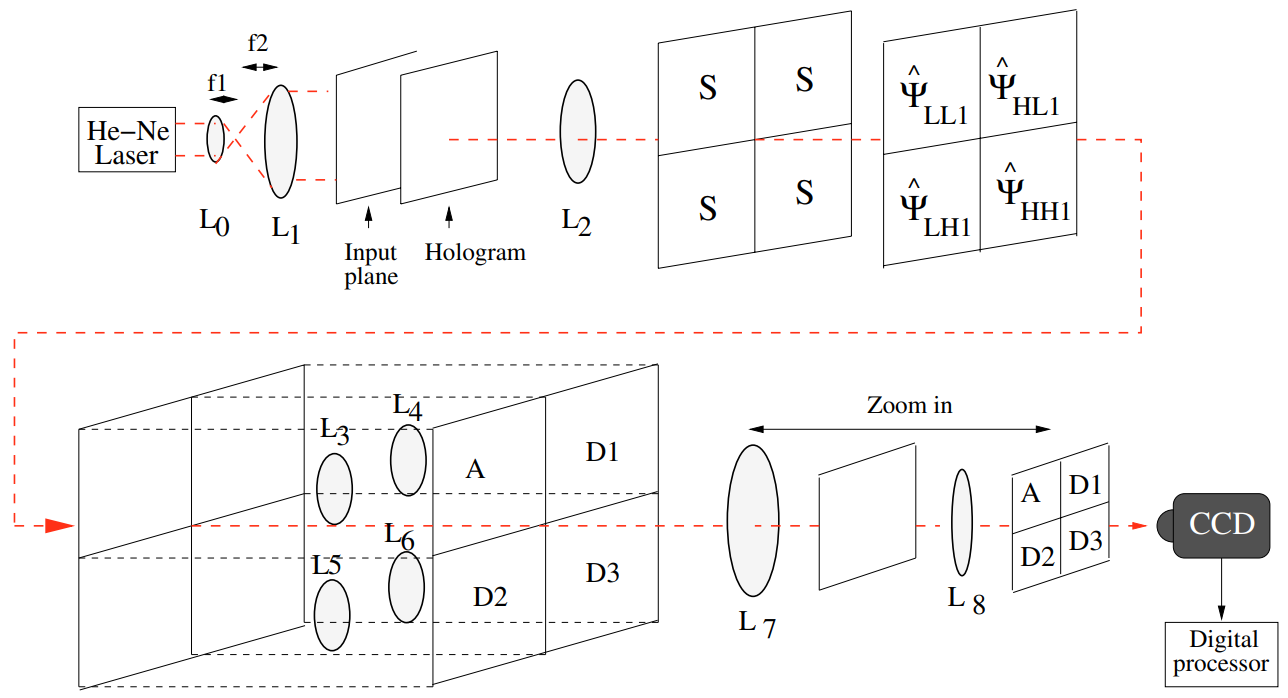
\includegraphics[width=0.8\linewidth]{figures/JPEG2000.png}}
	\caption{Оптическая схема реализации свёртки вейвлетами Хаара. Источник: \cite{alkholidi2008real}.}
	\label{ris:JPEG2000}
\end{figure}
\begin{figure}[htbp]
	\centering
		\begin{minipage}{.40\textwidth}
			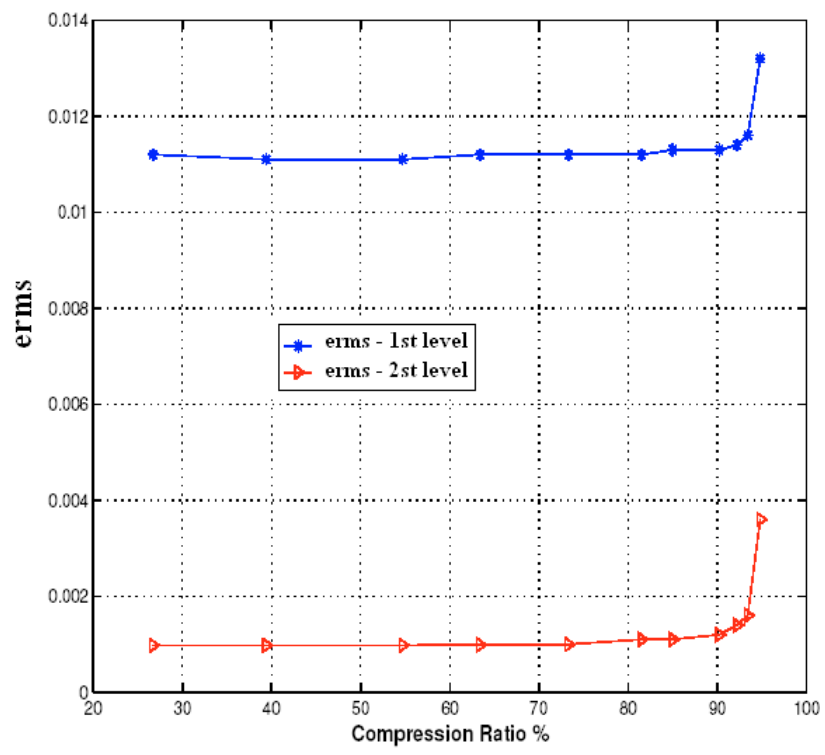
\includegraphics[width=\linewidth]{figures/VLCERMS.png}
			\label{ris:VLCERMS}
		\end{minipage}
		\hfill
		\begin{minipage}{.40\textwidth}
			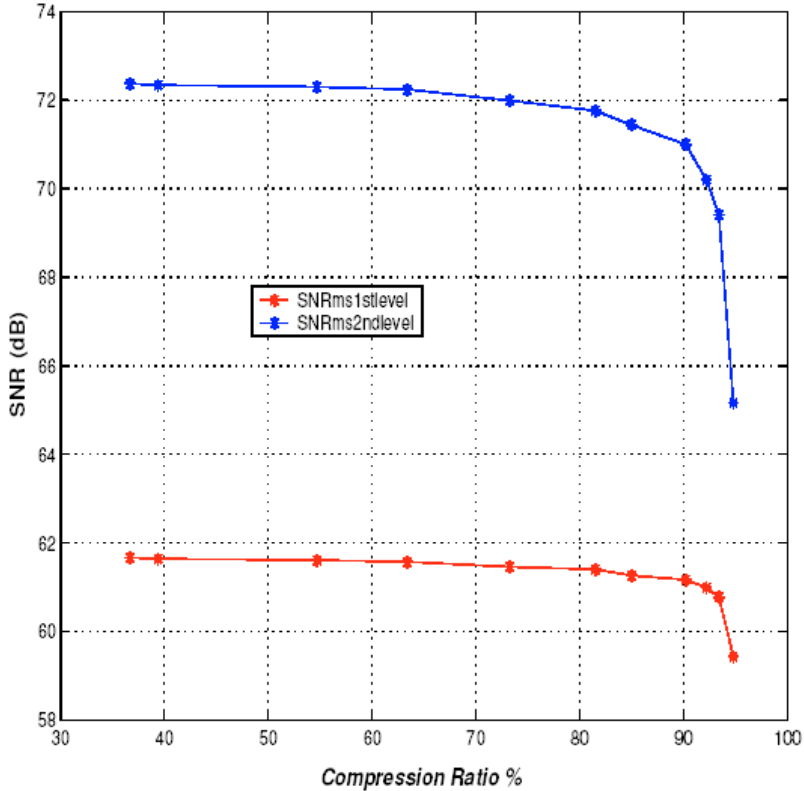
\includegraphics[width=0.95\linewidth]{figures/VLCSNR.png}
			\label{ris:VLCSNR}
		\end{minipage}
		\caption{Средне квадратичное отклонение значений пикселей и соотношения сигнал-шум в зависимости от степени сжатия метода с оптической свёрткой с вейвлетами Хаара \cite{alkholidi2008real}. Красная и синяя линии соответствую первому и второму уровню отношению размера ядра к размеру изображения. Источник: \cite{alkholidi2008real}.}
		\label{ris:VLCERMSSNR}
\end{figure}

\FloatBarrier\par
Ещё одна реализация основана на замене косинусного преобразованием в алгоритме JPEG оптической частью \cite{alkholidi2007new}. Основная идея заключается в отражении изображения по двум осям, приводя его к чётному виду и последующему получению Фурье образа с помощью линзы \cite{goodman2005introduction}, и последующего удаления определённых частот. Схема этого метода изображена на рисунке \ref{ris:JPEG}. Результаты численных расчётов представлены в таблице \ref{ris:JPEGres}. Результаты эксперимента для степени сжатия на рисунке \ref{ris:JPEGres2}.
\begin{figure}[htbp]
	\centering{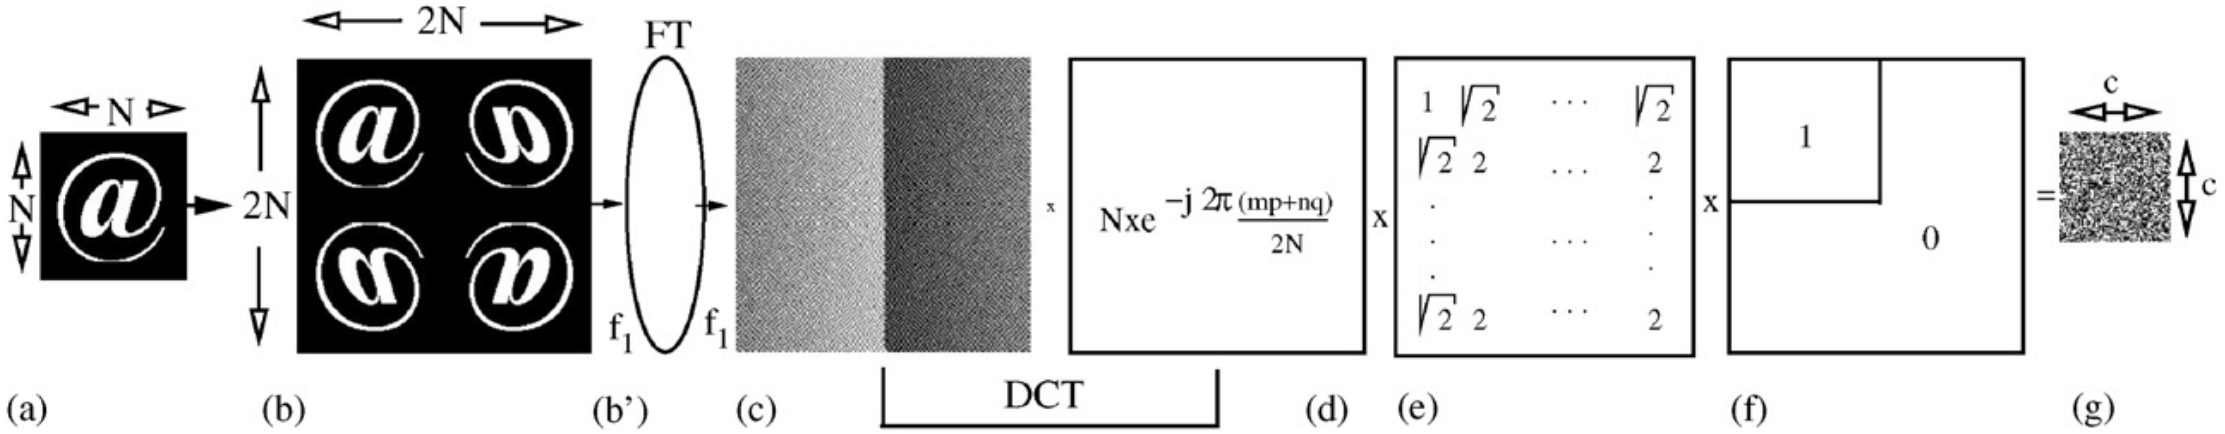
\includegraphics[width=0.8\linewidth]{figures/JPEG.png}}
	\caption{Принципиальная схема оптического косинусного преобразования и последующего обрезания частот. Источник: \cite{alkholidi2007new}.}
	\label{ris:JPEG}
\end{figure}
\begin{figure}[htbp]
	\centering{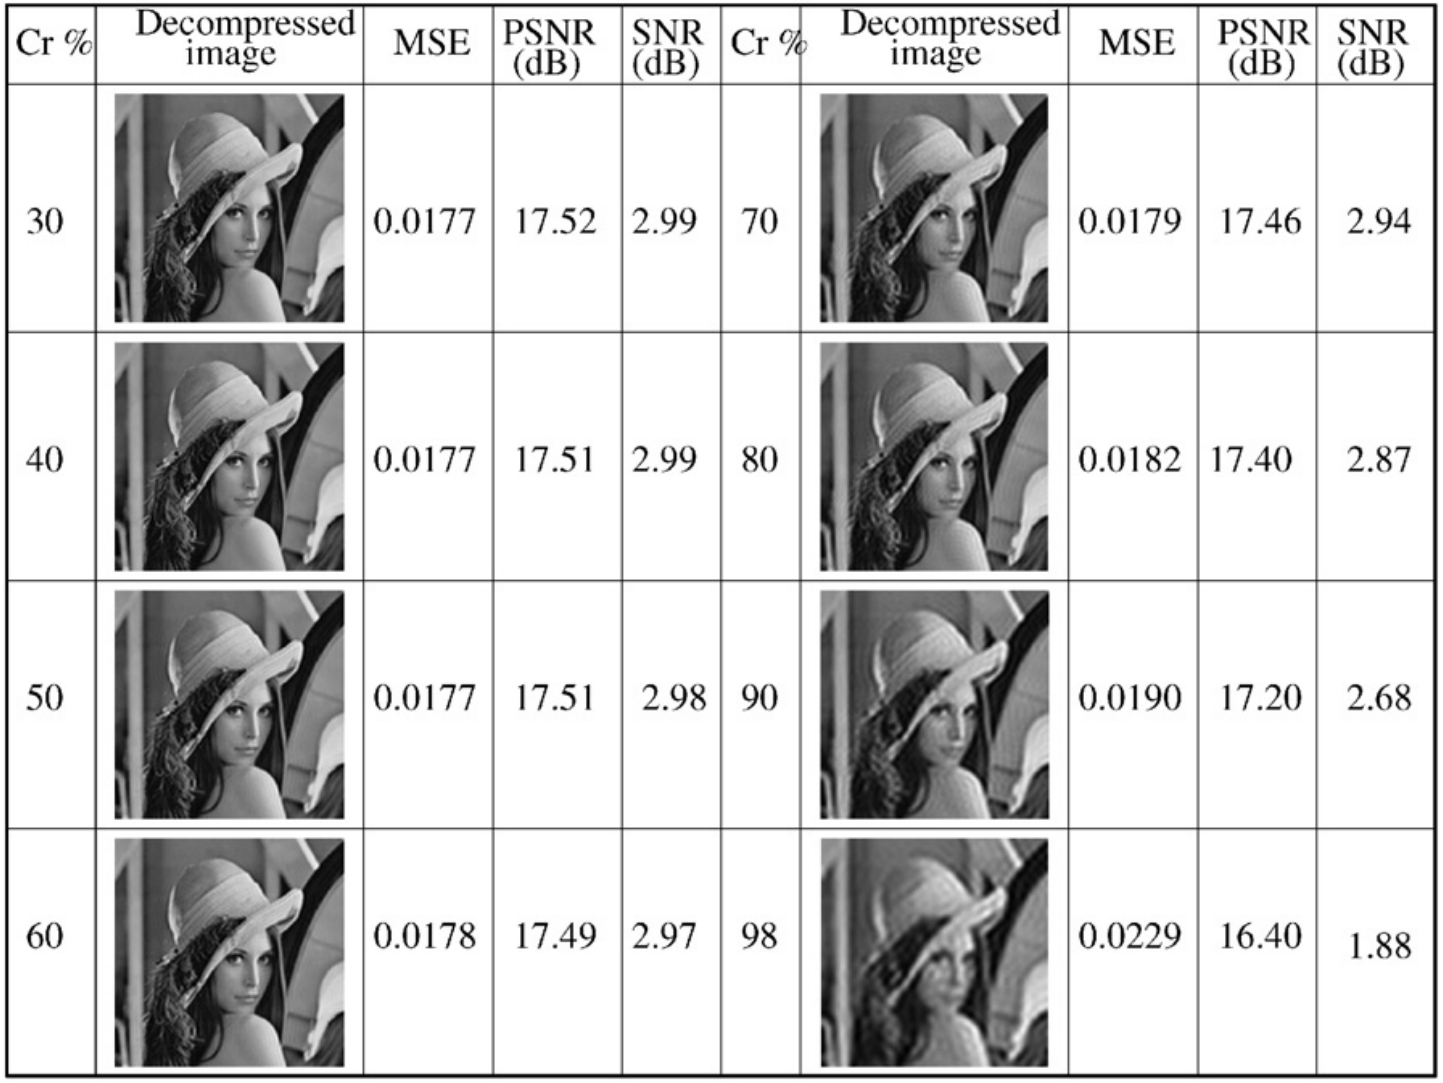
\includegraphics[width=0.7\linewidth]{figures/JPEGres.png}}
	\caption{Результаты симуляции сжатия изображения при помощи оптического косинусного преобразования и последующего восстановления. Источник: \cite{alkholidi2007new}.}
	\label{ris:JPEGres}
\end{figure}
\begin{figure}[htbp]
	\centering{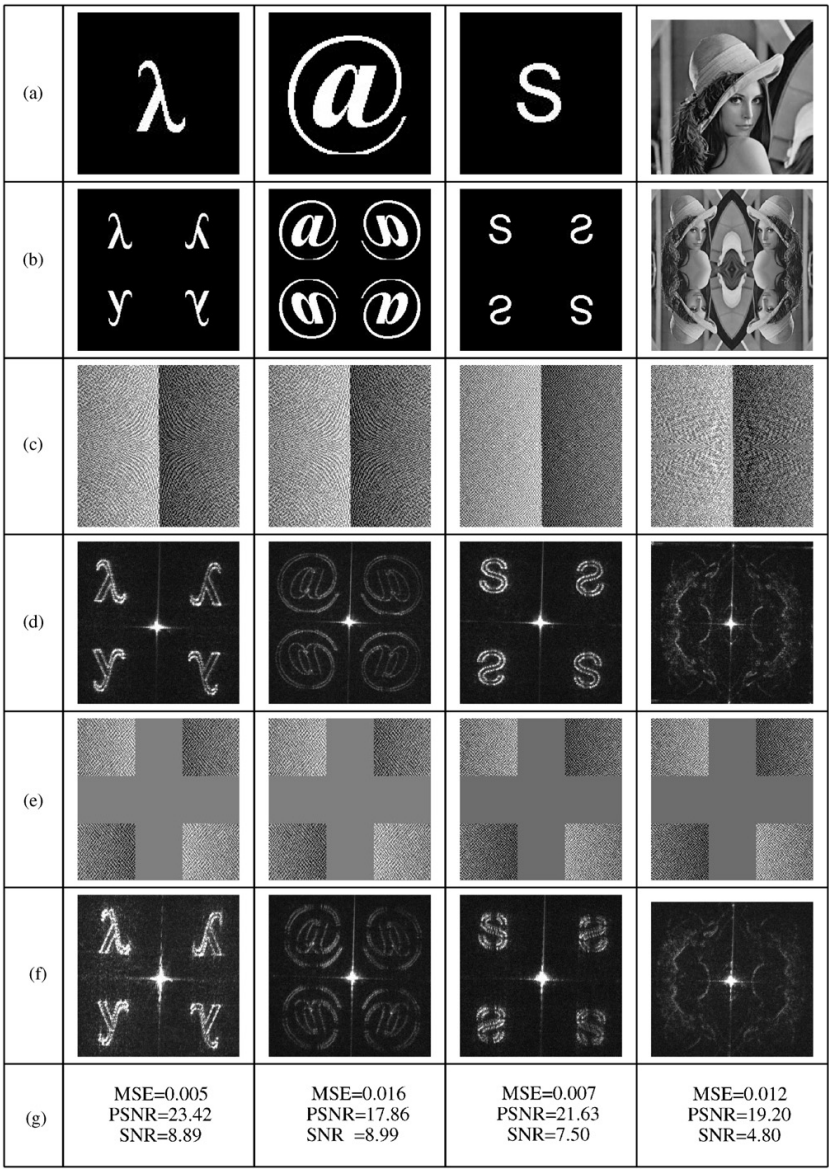
\includegraphics[angle=90,width=0.9\linewidth]{figures/JPEGres2.png}}
	\caption{Результаты оптической реализации сжатия и декомпрессии JPEG (Степень сжатия $50\%$): (a) исходное изображение; (b) реплицированное изображение; (c) реплицированный спектр изображения; (d) оптическая плоскость вывода; (e) сжатый спектр; (f) декомпрессированное изображение; (g) оценка между (b) и (f). Источник: \cite{alkholidi2007new}.}
	\label{ris:JPEGres2}
\end{figure}
Сравнивая численные расчёты на рисунке \ref{ris:JPEGres} и эксперимент на рисунке \ref{ris:JPEGres2} видно, что данный оптический метод сжатия очень плохо работает с не разреженными изображениями. Из этого сравнения дополнительно видно, что мера сравнения изображений не всегда соотносится с наблюдаемой разницей. Среднеквадратичная ошибка, для картинки в 1-ой строке, в эксперименте меньше, чем в симуляции для соответствующей степени сжатия $50\%$, но в эксперименте картинка восстановилась намного хуже.

\FloatBarrier\par
Ещё одна реализация -- использование JTC коррелятора для свёртки изображения со случайной матрицей \cite{velez2016optical} и последующее оптическое масштабирование этой свёртки, описанное в \cite{trejos2016optical}. Основа этого метода лежит в сжатии разреженных данных с помощью случайных проекций \cite{amador2007random}. Суть заключается в разложении изображения по случайным заранее заданным функциям. Результат численных расчётов работы этой схемы изображён на рисунке \ref{ris:RandomProjRes}.
\begin{figure}[htbp]
	\centering{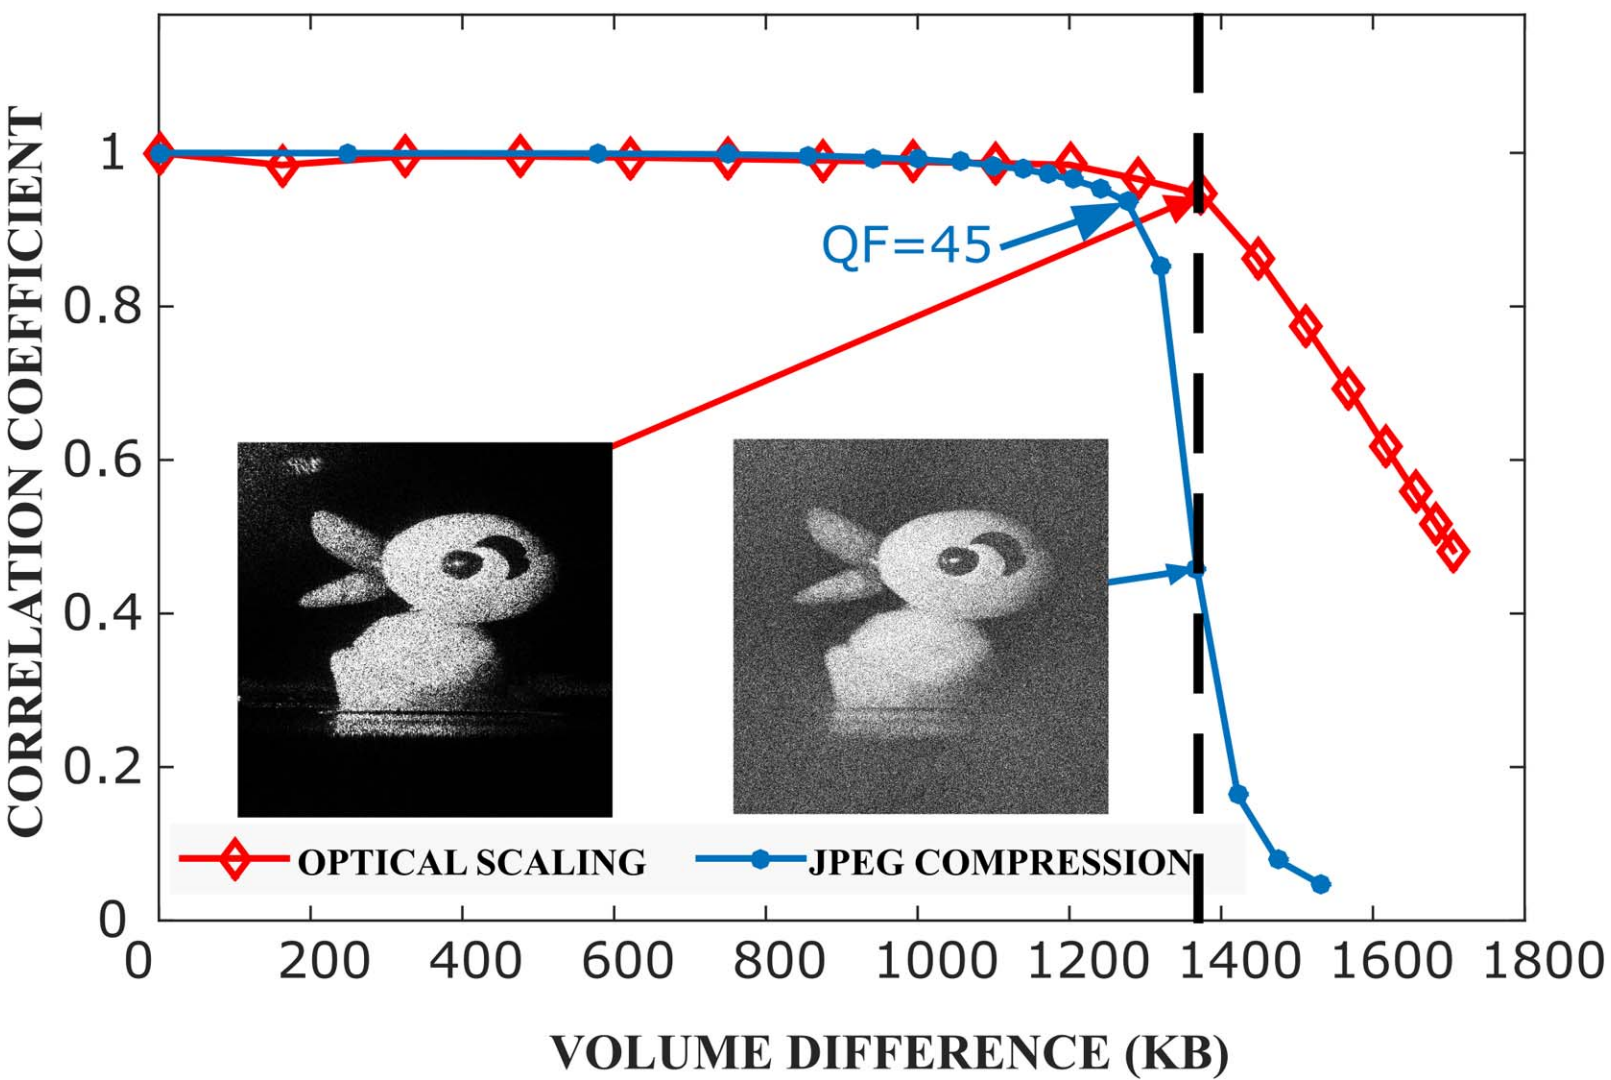
\includegraphics[width=0.8\linewidth]{figures/RandomProjRes.png}}
	\caption{Коэффициент корреляции между объектом, восстановленным из несжатых и сжатых данных поля для оптического масштабирования и сжатия JPEG, с точки зрения разницы в объеме. Источник: \cite{velez2016optical}.}
	\label{ris:RandomProjRes}
\end{figure}
График показывает, что при разнице размеров сжатого и несжатого изображения примерно в $1400$ КБайт, рассмотренный метод показал существенное превосходство над стандартным JPEG: коэффициент корреляции восстановленного с несжатым изображением $0.95$ у метода против $0.5$ у JPEG.





\paragraph{Дифракционные нейронные сети}
Дифракционная нейронная сеть представляет массив оптически неоднородных тонких масок. На каждой такой маске поточечно модулируется фаза и/или амплитуда поля. Система делится на исходную плоскость, где проецируется изображение, плоскости после масок и выходную плоскость. Такую систему ассоциируют с нейронной сетью типа перцептрон потому, что поле в каждой точки плоскости линейно связано с полями точек в предыдущей плоскости. Важным отличием является тот факт, что количество весов перехода между слоями намного меньше. Это связано с тем фактом, что поле в какой-то точке плоскости после маски, вычисляется как интеграл от умножения поля в предыдущей плоскости с фиксированным ядром, и последующего умножения этого числа на управляемый коэффициент. Математическое описание представлено уравнением \ref{eq:FieldProp}.
\begin{equation}\label{eq:FieldProp}
	u_i(x,y) = w_i(x,y)\int\limits_{-\infty}^{+\infty}\int\limits_{-\infty}^{+\infty}u_{i-1}(\xi,\eta)\frac{e^{ik\sqrt{L^2+(x-\xi)^2+(y-\eta)^2}}}{\sqrt{L^2+(x-\xi)^2+(y-\eta)^2}} d\xi d\eta.
\end{equation}
В этом уравнение $u_i,u_{i-1}$ -- поле в текущем и предыдущем слое соответственно, $L$ -- расстояние между слоями, $w_i(x,y)$ -- вес нейрона в точке $x,y$, а количество нейронов и дискретизация этого уравнения определяется степенью точности, с которой можно создавать оптические неоднородности.
Таким образом, на один переход между слоями размером $N$ нейронов, перцептрон имеет $N^2$ весов, а дифракционная нейронная сеть -- $N$.

\FloatBarrier\par
Классическая реализация дифракционной нейронной сети представлена в \cite{qian2020performing}. На рисунке \ref{ris:ClassicD2NN} изображена оптическая схема эксперимента. В этой работе использовалось излучение с длинной волны $17.6$ мм. Оптическая нейронная сеть выполняла логические операции (НЕ, И, ИЛИ). Выбор операции и двух входных сигналов производился за счёт первой плоскости, далее шли два скрытых слоя, состоящих из параллелепипедов различной высоты, которая определяет фазовую задержку, создаваемую этим элементом. На выходной плоскости значениям $0$ и $1$ соответствовали две разные области фокусировки. Высота каждого параллелепипеда оптимизировалась с помощью методов машинного обучения. 
\begin{figure}[htbp]
	\centering{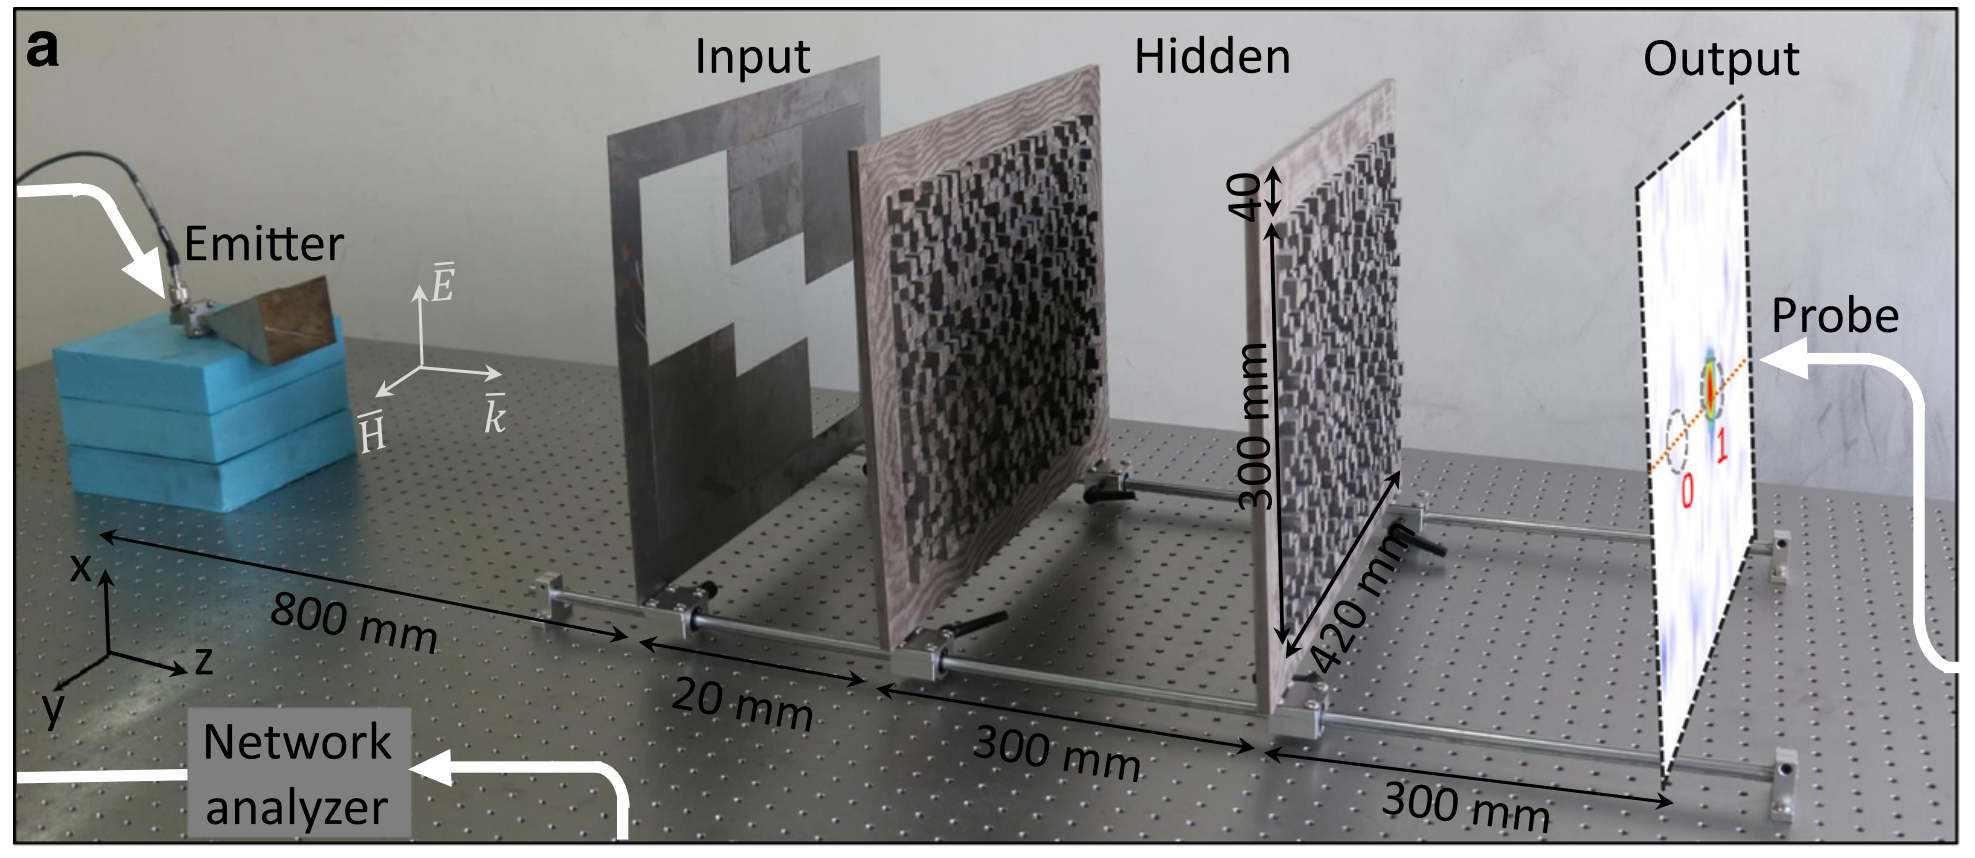
\includegraphics[width=0.8\linewidth]{figures/ClassicD2NN.png}}
	\caption{Экспериментальная реализация дифракционной нейронной сети из статьи \cite{qian2020performing}. Источник: \cite{qian2020performing}.}
	\label{ris:ClassicD2NN}
\end{figure}
После обучения, нейронная сеть корректно выполняла, описанные выше, логические операции.

\FloatBarrier\par
Сравнение более сложных реализаций представлено в статье \cite{yan2019fourier}. Архитектуры, протестированные в этой работе, представлены на рисунке \ref{ris:FD2NN} в схематическом виде. Сеть обучалась классификации рукописных цифр и должна была сфокусировать результирующее поле в один из десяти детекторов, соответствующих цифрам $0$--$9$. На этом же рисунке представлены графики результатов их обучения.
\begin{figure}[htbp]
	\centering{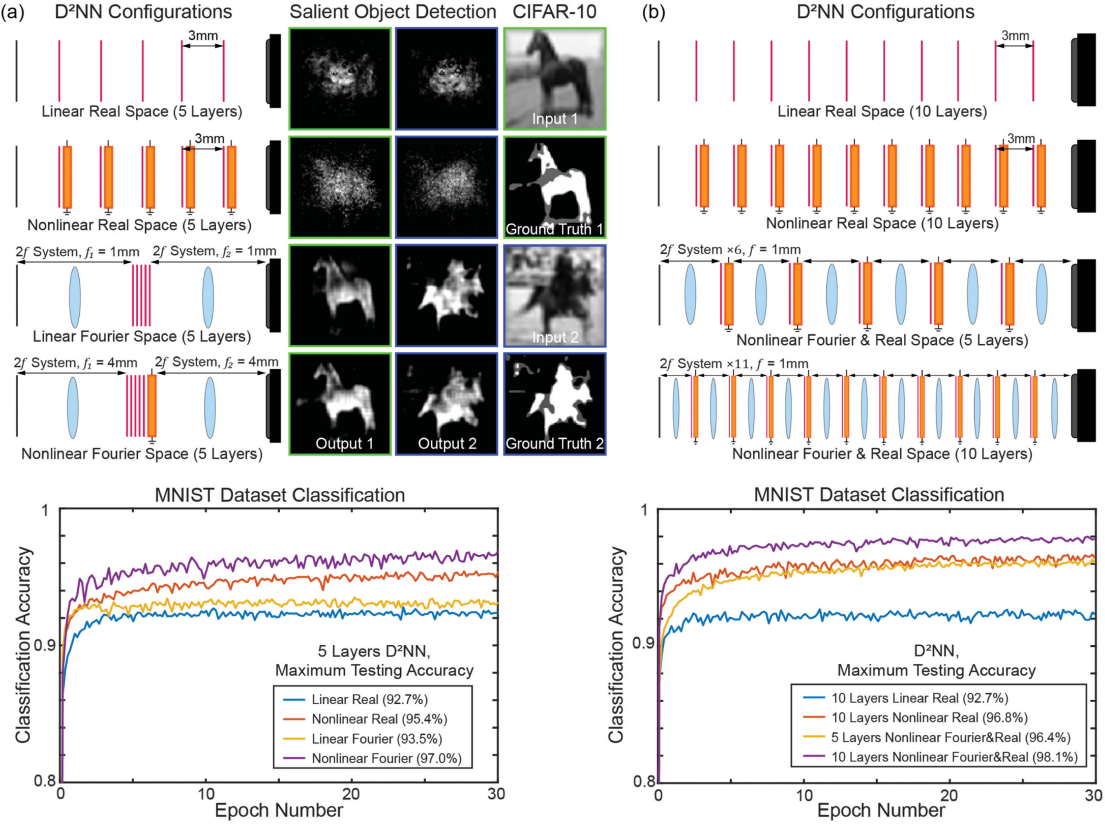
\includegraphics[width=0.8\linewidth]{figures/FD2NN.png}}
	\caption{Схемы дифракционных нейронных сетей (сверху) и результаты их обучения (снизу). Источник: \cite{yan2019fourier}.}
	\label{ris:FD2NN}
\end{figure}





% \paragraph{Гибридные оптоэлектронные сети}

